\documentclass[aps,prb,onecolumn,amssymb,amsmath,superscriptaddress]{revtex4-1}
\usepackage{bm}
\usepackage{times}
\usepackage{graphicx}
\usepackage{color}
\usepackage{amsmath}
\usepackage{braket}
\usepackage{dcolumn}
\usepackage[colorlinks=true, letterpaper=true, pdfstartview=FitV, linkcolor=blue, citecolor=blue, urlcolor=blue]{hyperref}
\usepackage{appendix}
\usepackage[normalem]{ulem}
\usepackage{cancel}
% \usepackage{geometry}
% \geometry{a4paper,scale=0.8}
% \usepackage{caption}
% \captionsetup{font={scriptsize}}

\begin{document}

\title{NEGF Notes}
\author{Li Gaoyang}
% \date{}
\date{\today}
\maketitle
% \tableofcontents

% \newpage

\subsection{Hamiltonian}
\begin{equation}
H=H_{L}+H_{R}+H_{d}+H_{T}+H_{s d}
\end{equation}
\begin{equation}
H_{L}=\sum_{k \sigma} \epsilon_{k \sigma, L} c_{k \sigma}^{\dagger} c_{k \sigma}
\end{equation}
\begin{equation}
H_{R}=\sum_{q} \omega_{q} a_{q}^{\dagger} a_{q}
\end{equation}
\begin{equation}
H_{d}=\sum_{n \sigma} \epsilon_{n \sigma} d_{n \sigma}^{\dagger} d_{n \sigma}
\end{equation}
\begin{equation}
H_{T}=\sum_{k \sigma n}\left(t_{k \sigma n} c_{k \sigma}^{\dagger} d_{n \sigma}+t_{k \sigma n}^{*} d_{n \sigma}^{\dagger} c_{k \sigma}\right)
\end{equation}
\begin{equation}
H_{s d}=-\sum_{q n m} J_{q}\left(d_{n \uparrow}^{\dagger} d_{m \downarrow} a_{q}^{\dagger}+a_{q} d_{m \downarrow}^{\dagger} d_{n \uparrow}\right) \delta\left(\epsilon_{n \uparrow}-\epsilon_{m \downarrow}-\omega_{q}\right)
\end{equation}
\begin{equation}
s_{q}^{+}=\sum_{n m} d_{n \uparrow}^{\dagger} d_{m \downarrow} \delta_{\uparrow \downarrow}
\end{equation}
\begin{equation}
s_{q}^{-}=\sum_{n m} d_{m \downarrow}^{\dagger} d_{n \uparrow} \delta_{\uparrow \downarrow}
\end{equation}
\subsubsection{check operators}
\begin{equation}
i \dot{a}_{q}=\omega_{q} a_{q}-J_{q} s_{q}^{+}
\end{equation}
\begin{equation}
i \dot{c}_{k \sigma}=\epsilon_{k \sigma, L} c_{k \sigma}+\sum_{k^{\prime}} t_{k \sigma n} d_{n \sigma}
\end{equation}
\begin{equation}
i \dot{d}_{n \uparrow}=\epsilon_{n \uparrow} d_{n \uparrow}+\sum_{k} t_{k \uparrow n}^{*} c_{k \uparrow}-\sum_{q, m} J_{q} a_{q}^{\dagger}d_{m \downarrow}\delta(\epsilon_{n \uparrow}-\epsilon_{m \downarrow}-\omega_{q})
\end{equation}
\begin{equation}
i \dot{d}_{n \downarrow}=\epsilon_{n \downarrow} d_{n \downarrow}+\sum_{k} t_{k \downarrow n}^{*} c_{k \downarrow}-\sum_{q, m} J_{q} a_{q}d_{m \uparrow}\delta(\epsilon_{m \uparrow}-\epsilon_{n \downarrow}-\omega_{q})
\end{equation}
\subsection{spin current ???}
Define
\begin{equation}
G_{d, R}\left(\tau, \tau^{\prime}\right)=-i\langle s_{q}^{+}(\tau) a_{q}^{\dag}(\tau')\rangle.
\end{equation}
The lesser Green's function is($s_{q}^{+}$ is fermionic but $a_{q}$ is bosonic)
\begin{equation}
G_{d, R}^{<}\left(t, t'\right)=-i\langle  a_{q}^{\dag}(t') s_{q}^{+}(t) \rangle
\end{equation}
We also define the Green’s function that is related to the QD (not the Green’s function of the QD),
\begin{equation}
G_{d}\left(\tau, \tau^{\prime}\right)= -i\left\langle T_{c} S s_{q}^{+}(\tau) s_{q}^{-}\left(\tau^{\prime}\right)\right\rangle .
\end{equation}
We have
\begin{equation}
-i \partial_{\tau^{\prime}} G_{d, R}\left(\tau, \tau^{\prime}\right)=\omega_{q} G_{d, R}\left(\tau, \tau^{\prime}\right)-J_{q} G_{d}
\end{equation}
or
\begin{equation}
G_{d, R} g_{R q}^{-1}=-J_{q} G_{d}
\end{equation}
or
\begin{equation}
G_{d, R}\left(\tau, \tau^{\prime}\right)=-J_{q} \int G_{d}\left(\tau, \tau_{1}\right) g_{R q}\left(\tau_{1}, \tau^{\prime}\right) d \tau_{1}
\end{equation}
the minus before $J_{q}$ originates from the minus in $H_{sd}$. The rules of analytic continuation gives
\begin{equation}
G_{d, R}^{<}\left(t, t^{\prime}\right)=-J_{q} \int_{-\infty}^{\infty}dt_{1} [G_{d}^{r}\left(t, t_{1}\right) g_{R q}^{<}\left(t_{1}, t^{\prime}\right) + G_{d}^{<}\left(t, t_{1}\right) g_{R q}^{a}\left(t_{1}, t^{\prime}\right)]
\end{equation}
and
\begin{equation}
G_{R,d}^{<}\left(t, t^{\prime}\right)=-J_{q} \int_{-\infty}^{\infty}dt_{1} [g_{R q}^{r}\left(t, t_{1}\right) G_{d}^{<}\left(t_{1}, t'\right)  + g_{R q}^{<}\left(t, t_{1}\right) G_{d}^{a}\left(t_{1}, t'\right)]
\end{equation}
The spin current flows out of right lead is
\begin{equation}
\begin{split}
I_{s}&= i \sum_{q} J_{q}\left(\left\langle s_{q}^{+} a_{q}^{\dagger}\right\rangle-\left\langle a_{q} s_{q}^{-}\right\rangle\right) \\
&=-\sum_{q}J_{q}(G_{d,R}^{<}(t,t)-G_{R,d}^{<}(t,t)) \\
&=2\rm{Re}\sum_{q} \int  d t_{1}\operatorname{Tr}\left[G_{d}^{r}\left(t, t_{1}\right) \Sigma_{Rq}^{<}\left(t_{1}, t^{\prime}\right)+G_{d}^{<}\left(t, t_{1}\right) \Sigma_{Rq}^{a}\left(t_{1}, t^{\prime}\right)\right]
% \\ &=2\rm{Re}\sum_{q} \int  d t_{1}\operatorname{Tr}\left[\left(G_{d}^{>}-G_{d}^{<}\right) \Sigma_{R q}^{<}+G_{d}^{<}\left(\Sigma_{R q}^{a}-\Sigma_{R q}^{r}\right)\right]
\end{split}
\end{equation}
\begin{equation}
\Sigma_{Rq}^{\gamma}(\tau, \tau')=J_{q}^{2}g_{Rq}^{\gamma}(\tau, \tau')
\end{equation}
\subsection{Calculation of $G_{d}$}
Definition:
\begin{equation}
\begin{split}
G_{d}\left(\tau, \tau^{\prime}\right)&=
-i\left\langle T_{c} S s_{q}^{+}(\tau) s_{q}^{-}\left(\tau^{\prime}\right)\right\rangle \\
&=-i\sum_{mnm'n'}\langle T_{c}S d_{n \uparrow}^{\dagger} d_{m \downarrow} d_{m' \downarrow}^{\dagger} d_{n' \uparrow} \rangle \delta\left(\epsilon_{n \uparrow}-\epsilon_{m \downarrow}-\omega_{q}\right) \delta\left(\epsilon_{n' \uparrow}-\epsilon_{m' \downarrow}-\omega_{q}\right) 
\end{split}
\end{equation}
When right lead is absent, the system Hamiltonian is
\begin{equation}
H = H_{L} + H_{d} + H_{T}.
\end{equation}
\begin{equation}
G_{d}\left(\tau, \tau^{\prime}\right)=-i\sum_{mnm'n'}G_{L,n'n\uparrow}(\tau', \tau) G_{L,mm'\downarrow}(\tau, \tau') \delta\left(\epsilon_{n \uparrow}-\epsilon_{m \downarrow}-\omega_{q}\right) \delta\left(\epsilon_{n' \uparrow}-\epsilon_{m' \downarrow}-\omega_{q}\right)
\end{equation}
where
\begin{equation}
\begin{split}
G_{L,mn\sigma}(\tau, \tau')&= -i\langle T_{c}d_{m\sigma}(\tau) d_{n\sigma}^{\dag}(\tau')\rangle \\
&=g_{mn\sigma}(\tau, \tau')\delta_{mn} \\
&~~~+ \iint d\tau_{1}d\tau_{2} g_{mm\sigma}(\tau, \tau_{2}) \sum_{k} t_{k\sigma n}t_{k\sigma m}^{*} g_{k\sigma}(\tau_{2}, \tau_{1}) g_{nn\sigma}(\tau_{1}, \tau') \\
&~~~ +\cdots \\
&=g_{mn\sigma}(\tau, \tau')\delta_{mn} + \iint d\tau_{1}d\tau_{2} g_{mm\sigma}(\tau, \tau_{2}) \Sigma_{L,mn\sigma}(\tau_{2}, \tau_{1}) g_{nn\sigma}(\tau_{1}, \tau')\\
&~~~+ \cdots \\
&= 1 /\left[g_{mn \sigma}^{-1}-\Sigma_{L,mn \sigma}\right]
\end{split}
\end{equation}
\begin{equation}
g_{mn\sigma}(\tau, \tau') = -i\langle T_{c}d_{m\sigma}(\tau) d_{n\sigma}^{\dag}(\tau')\rangle_{0}
\end{equation}
Self-energy of left lead
\begin{equation}
\Sigma_{L,mn\sigma}(\tau_{2}, \tau_{1}) = \sum_{k} t_{k\sigma n}t_{k\sigma m}^{*} g_{k\sigma}(\tau_{2}, \tau_{1})
\end{equation}
where
\begin{equation}
g_{k\sigma}(\tau_{2}, \tau_{1}) = -i\langle T_{c}c_{k\sigma}(\tau_{2}) c_{k\sigma}^{\dag}(\tau_{1})\rangle_{0}.
\label{eq:left-self-energy}
\end{equation}
When left lead is absent, system Hamiltonian is
\begin{equation}
H = H_{d} + H_{R} + H_{sd}.
\end{equation}
\begin{equation}
\begin{split}
G_{d}\left(\tau, \tau^{\prime}\right) =&-i\sum_{mn} g_{n \uparrow}\left(\tau^{\prime}, \tau\right) g_{m \downarrow}\left(\tau, \tau^{\prime}\right) \delta(\varepsilon_{n\uparrow} - \varepsilon_{m\downarrow} - \omega_{q})\\
&-\int d\tau_{1}\int d\tau_{2} \sum_{mnm'n'}g_{n \uparrow}\left(\tau_{1}, \tau\right) g_{m \downarrow}\left(\tau, \tau_{1}\right) \Sigma_{R,mnm'n' }\left(\tau_{1}, \tau_{2}\right) g_{n'\uparrow}\left(\tau^{\prime}, \tau_{2}\right)g_{m'\downarrow}(\tau_{2}, \tau') \\
&~~~\times \delta(\varepsilon_{n\uparrow} - \varepsilon_{m\downarrow} - \omega_{q_{1}})\delta(\varepsilon_{n'\uparrow} - \varepsilon_{m'\downarrow} - \omega_{q_{1}})\\
& + \cdots \\
=& g_{d}(\tau, \tau') + \iint d\tau_{1}d\tau_{2}g_{d}(\tau, \tau_{1}) \Sigma_{R}(\tau_{1}, \tau_{2}) G_{d}(\tau_{2}, \tau')
\end{split}
\end{equation}
in which, 
\begin{equation}
g_{d}\left(\tau, \tau^{\prime}\right) = -i\sum_{mn} g_{n \uparrow}\left(\tau^{\prime}, \tau\right) g_{m \downarrow}\left(\tau, \tau^{\prime}\right) \delta(\varepsilon_{n\uparrow} - \varepsilon_{m\downarrow} - \omega_{q}),
\end{equation}
the self-energy of right lead is
\begin{equation}
\Sigma_{R,mnm'n'}(\tau_{1}, \tau_{2}) = \sum_{q1}J_{q_{1}}^{2} g_{Rq_{1}}(\tau_{1}, \tau_{2}) \delta(\varepsilon_{n\uparrow} - \varepsilon_{m\downarrow} - \omega_{q_{1}})\delta(\varepsilon_{n'\uparrow} - \varepsilon_{m'\downarrow} - \omega_{q_{1}})
\end{equation}
\begin{equation}
g_{Rq_{1}}(\tau_{1}, \tau_{2}) = -i\langle T_{c}a_{q_{1}}(\tau_{1}) a_{q_{1}}^{\dag}(\tau_{2})\rangle_{0}
\end{equation}
Hence, when both leads are present, we have
\begin{equation}
\begin{split}
G_{d}\left(\tau, \tau^{\prime}\right)=&-i \sum_{mnm'n'}G_{L,nn' \uparrow}\left(\tau^{\prime}, \tau\right) G_{L,mm' \downarrow}\left(\tau, \tau^{\prime}\right)\delta\left(\epsilon_{n \uparrow}-\epsilon_{m \downarrow}-\omega_{q}\right) \delta\left(\epsilon_{n' \uparrow}-\epsilon_{m' \downarrow}-\omega_{q}\right)\\
&-i \sum_{mnm'n'}G_{L,nn' \uparrow}\left(\tau_{1}, \tau\right) G_{L,mm' \downarrow}\left(\tau, \tau_{1}\right) \Sigma_{R,mnm'n'}\left(\tau_{1}, \tau_{2}\right) G_{d}\left(\tau_{2}, \tau^{\prime}\right) \delta\left(\epsilon_{n \uparrow}-\epsilon_{m \downarrow}-\omega_{q}\right)\\
&\qquad\times \delta\left(\epsilon_{n' \uparrow}-\epsilon_{m' \downarrow}-\omega_{q}\right)
\label{eq:1}
\end{split}
\end{equation}
For the sack of convenience, we rewrite the above formula in matrix presentation as follows(the matrix indices are QD level indices $m,n$, not corrected yet!), and omit energy conservation constrain.
\begin{equation}
{\color{red}{?}}~~G_{d}\left(\tau, \tau^{\prime}\right)=-i G_{L \uparrow}\left(\tau^{\prime}, \tau\right) G_{L \downarrow}\left(\tau, \tau^{\prime}\right)-i G_{L \uparrow}\left(\tau_{1}, \tau\right) G_{L \downarrow}\left(\tau, \tau_{1}\right) \Sigma_{R }\left(\tau_{1}, \tau_{2}\right) G_{d}\left(\tau_{2}, \tau^{\prime}\right)
\end{equation}
\subsection{continuation on Eq.(\ref{eq:1})}
\begin{eqnarray}
% \center
A(\tau_{1}, \tau') \equiv\int d\tau_{2}\Sigma_{R }\left(\tau_{1}, \tau_{2}\right) G_{d}\left(\tau_{2}, \tau^{\prime}\right)\\
B(\tau, \tau_{1}) \equiv G_{L \uparrow}\left(\tau_{1}, \tau\right) G_{L \downarrow}\left(\tau, \tau_{1}\right)\\
C(\tau, \tau')\equiv -i G_{L \uparrow}\left(\tau_{1}, \tau\right) G_{L \downarrow}\left(\tau, \tau_{1}\right) A(\tau_{1}, \tau') \rightarrow \\
C(\tau, \tau') = -i\int d\tau_{1}B(\tau, \tau_{1})A(\tau_{1}, \tau')\\
D(\tau, \tau') \equiv -i G_{L \uparrow}\left(\tau^{\prime}, \tau\right) G_{L \downarrow}\left(\tau, \tau^{\prime}\right)
\end{eqnarray}
So, we have
\begin{equation}
G_{d}(\tau, \tau') = D + C
\end{equation}
Using the analytic continuation theorem, we have
\begin{equation}
D^{<} = -i G_{L \uparrow}^{>} G_{L \downarrow}^{<}
\end{equation}
\begin{equation}
C^{<}=-i(B^{r} A^{<}+B^{<} A^{a})
\end{equation}
where
\begin{equation}
B^{r} = G_{L \uparrow}^{a} G_{L \downarrow}^{<}+G_{L \uparrow}^{>} G_{L \downarrow}^{r}+G_{L \uparrow}^{a} G_{L \downarrow}^{r}
\end{equation}
\begin{equation}
A^{<}=\Sigma_{R}^{r} G_{d}^{<}+\Sigma_{R}^{<} G_{d}^{a}
\end{equation}
\begin{equation}
B^{<}=G_{L\uparrow}^{>} G_{L\downarrow}^{<}
\end{equation}
\begin{equation}
A^{a}=\Sigma_{R}^{a} G_{d}^{a}
\end{equation}
Then, the analytic continuation theorem on Eq.(\ref{eq:1}) yields
\begin{equation}
G_{d}^{<}=-i G_{L \uparrow}^{>} G_{L \downarrow}^{<} -i\left[(G_{L \uparrow}^{a} G_{L \downarrow}^{<}+G_{L \uparrow}^{>} G_{L \downarrow}^{r}+G_{L \uparrow}^{a} G_{L \downarrow}^{r})(\Sigma_{R}^{r} G_{d}^{<}+\Sigma_{R}^{<} G_{d}^{a}) + (G_{L\uparrow}^{>} G_{L\downarrow}^{<})(\Sigma_{R}^{a} G_{d}^{a})\right]
\label{eq:Gd<}
\end{equation}
Similarly, 
\begin{equation}
\begin{split}
C^{r}&=-iB^{r} A^{r} \\
&=-i(G_{L \uparrow}^{a} G_{L \downarrow}^{<}+G_{L \uparrow}^{>} G_{L \downarrow}^{r}+G_{L \uparrow}^{a} G_{L \downarrow}^{r})(\Sigma_{R}^{r} G_{d}^{r})
\end{split}
\end{equation}
\begin{equation}
D^{r}=-i(G_{L \uparrow}^{a} G_{L \downarrow}^{<}+G_{L \uparrow}^{>} G_{L \downarrow}^{r}+G_{L \uparrow}^{a} G_{L \downarrow}^{r}),
\end{equation}
we have
\begin{equation}
\begin{split}
G_{d}^{r} &=  -i(G_{L \uparrow}^{a} G_{L \downarrow}^{<}+G_{L \uparrow}^{>} G_{L \downarrow}^{r}+G_{L \uparrow}^{a} G_{L \downarrow}^{r})-i(G_{L \uparrow}^{a} G_{L \downarrow}^{<}+G_{L \uparrow}^{>} G_{L \downarrow}^{r}+G_{L \uparrow}^{a} G_{L \downarrow}^{r})(\Sigma_{R}^{r} G_{d}^{r}) \\
&=\frac{-i\left(G_{L \uparrow} G_{L \downarrow}\right)^{r}}{ 1+i\left(G_{L \uparrow} G_{L \downarrow}\right)^{r} \Sigma_{R}^{r}}
\end{split}
\end{equation}
\begin{equation}
(G_{L \uparrow} G_{L \downarrow})^{r} \equiv G_{L \uparrow}^{a} G_{L \downarrow}^{<}+G_{L \uparrow}^{>} G_{L \downarrow}^{r}+G_{L \uparrow}^{a} G_{L \downarrow}^{r}
\end{equation}
Now we calculate $G_{d}^{a}$.
\begin{equation}
C^{a}=-iB^{a} A^{a}
\end{equation}
\begin{equation}
B^{a}=G_{L \uparrow}^{r} G_{L \downarrow}^{<}+G_{L \uparrow}^{>} G_{L \downarrow}^{a}+G_{L \uparrow}^{r} G_{L \downarrow}^{a}
\end{equation}
\begin{equation}
D^{a}=-i(G_{L \uparrow}^{r} G_{L \downarrow}^{<}+G_{L \uparrow}^{>} G_{L \downarrow}^{a}+G_{L \uparrow}^{r} G_{L \downarrow}^{a})
\end{equation}
So we have
\begin{equation}
G_{d}^{a} = -i(G_{L \uparrow}^{r} G_{L \downarrow}^{<}+G_{L \uparrow}^{>} G_{L \downarrow}^{a}+G_{L \uparrow}^{r} G_{L \downarrow}
^{a})-i(G_{L \uparrow}^{r} G_{L \downarrow}^{<}+G_{L \uparrow}^{>} G_{L \downarrow}^{a}+G_{L \uparrow}^{r} G_{L \downarrow}^{a})(\Sigma_{R}^{a} G_{d}^{a})
\end{equation}
From Eq.(\ref{eq:Gd<}) we have
\begin{equation}
\begin{split}
G_{d}^{<}&=-i G_{L \uparrow}^{>} G_{L \downarrow}^{<}\left(1+\Sigma_{R}^{a} G_{d}^{a}\right)-i\left(G_{L \uparrow} G_{L \downarrow}\right)^{r}\left(\Sigma_{q}^{<} G_{d}^{a}+\Sigma_{R}^{r} G_{d}^{<}\right)\\
&=\frac{-i G_{L \uparrow}^{>} G_{L \downarrow}^{<}\left(1+\Sigma_{R}^{a} G_{d}^{a}\right) - i\left(G_{L \uparrow} G_{L \downarrow}\right)^{r}\Sigma_{R}^{<} G_{d}^{a}}{1+i\left(G_{L \uparrow} G_{L \downarrow}\right)^{r}\Sigma_{R}^{r}} \\
&=\frac{-i G_{L \uparrow}^{>} G_{L \downarrow}^{<}\left(1+\Sigma_{R}^{a} G_{d}^{a}\right)}{1+i\left(G_{L \uparrow} G_{L \downarrow}\right)^{r}\Sigma_{R}^{r}} + G_{d}^{r}\Sigma_{R}^{<} G_{d}^{a}\\
&=-i(G_{d}^{r}\Sigma_{R}^{r}+1) G_{L \uparrow}^{>} G_{L \downarrow}^{<}\left(1+\Sigma_{R}^{a} G_{d}^{a}\right) + G_{d}^{r}\Sigma_{R}^{<} G_{d}^{a}
\end{split}
\end{equation}
Similarly,
\begin{equation}
G_{d}^{>}=-i\left(G_{d}^{r} \Sigma_{R}^{r}+1\right) G_{L \uparrow}^{<} G_{L \downarrow}^{>}\left(1+\Sigma_{R}^{a} G_{d}^{a}\right)+G_{d}^{r} \Sigma_{R}^{>} G_{d}^{a}
\end{equation}
\subsection{DC spin current}

\begin{equation}
I_{s}= 2\rm{Re}\sum_{q} \int  \frac{dE}{2\pi}\operatorname{Tr}\left[\left(G_{d}^{>}-G_{d}^{<}\right) \Sigma_{R q}^{<}+G_{d}^{<}\left(\Sigma_{R q}^{a}-\Sigma_{R q}^{r}\right)\right]
\label{eq:current1}
\end{equation}

We have
\begin{equation}
G_{d}^{>}(E)-G_{d}^{<}(E)=-i\left(G_{d}^{r} \Sigma_{R}^{r}+1\right)\left(G_{L \uparrow}^{<} G_{L \downarrow}^{>}-G_{L \uparrow}^{>} G_{L \downarrow}^{<}\right)\left(1+\Sigma_{R}^{a} G_{d}^{a}\right)+G_{d}^{r}\left(\Sigma_{R}^{>}-\Sigma_{R}^{<}\right) G_{d}^{a}
\end{equation}
Fourier transformation
\begin{equation}
G_{d}^{<}(E) = \int_{-\infty}^{+\infty} dt G_{d}^{<}(t-t')e^{iE(t-t')}
\end{equation}
and inverse Fourier transformation
\begin{equation}
G_{d}^{<}(t-t') = \frac{1}{2\pi}\int_{-\infty}^{+\infty} d\omega G_{d}^{<}(E)e^{-iE(t-t')},
\end{equation}
are used, since the Green's functions only dependent on time difference. Then using Keldysh equation, we have
\begin{equation}
  \label{eq:3}
G_{L,mn\sigma}^{<}(E) = G_{L,mn\sigma}^{r}\Sigma_{L,mn\sigma}^{<}(E) G_{L,mn\sigma}^{a}(E),
\end{equation}
where $G_{L,mn\sigma}$ is the Green's function when left free lead, QD and left coupling present.  $\Sigma_{L,mn\sigma}^{<}$ is self-energy of left lead, defined in Eq. (\ref{eq:left-self-energy})
\begin{equation}
\Sigma_{L,mn\sigma}^{<} = if_{L\sigma}(E) \Gamma_{L,mn\sigma}(E).
\end{equation}
so,
\begin{equation}
G_{L,mn\sigma}^{<}(E) = iG_{L,mn\sigma}^{r}f_{L\sigma}(E) \Gamma_{L,mn\sigma}(E) G_{L,mn\sigma}^{a}(E)  \equiv i D_{L \sigma} f_{L \sigma},
\end{equation}
and
\begin{equation}
\begin{split}
G_{L,mn\sigma}^{>}(E) &= -(G_{L,mn\sigma}^{<}(E))^{\dag} \\
&= G_{L,mn\sigma}^{r}(E)\Sigma_{L,mn\sigma}^{>}(E) G_{L,mn\sigma}^{a}(E)\\
&=iD_{L\sigma}(f_{L\uparrow}(E) - 1)
\end{split}
\end{equation}
in which, $D_{L\sigma} = G_{L\sigma}^{r}\Gamma_{L\sigma}G_{L\sigma}^{a}$, thus
\begin{equation}
\begin{split}
G_{L\sigma}^{<} G_{L\sigma}^{>} - G_{L\sigma}^{>} G_{L\sigma}^{<} &= D_{L\uparrow}D_{L\downarrow} [(f_{L\uparrow}-1)f_{L\downarrow} - (f_{L\downarrow}-1) f_{L\uparrow}] \\
&= D_{L\uparrow}D_{L\downarrow} (f_{L\uparrow} - f_{L\downarrow})
\end{split}
\end{equation}
\begin{equation}
\begin{split}
\Sigma_{R}^{<}(E) &=  \sum_{q_{1}}J_{q_{1}}^{2} g_{Rq_{1}}^{<}(E) \\
&= if_{R}^{B}(E) \Gamma_{R}(E)
\end{split}
\end{equation}
\begin{equation}
\Sigma_{R}^{a} - \Sigma_{R}^{r} = \Sigma_{R}^{<} - \Sigma_{R}^{>} = i\Gamma_{R}(E).
\end{equation}
\begin{equation}
G_{d}^{>}-G_{d}^{<}=-i\left[f_{L \uparrow}-f_{L \downarrow}\right]\left(G_{d}^{r} \Sigma_{R q}^{r}+1\right) D_{L \uparrow} D_{L \downarrow}\left(1+\Sigma_{R q}^{a} G_{d}^{a}\right)-i G_{d}^{r} \Gamma_{R q} G_{d}^{a}
\end{equation}
\begin{equation}
\begin{aligned}
\left(G_{d}^{>}-G_{d}^{<}\right) \Sigma_{R q}^{<}+G_{d}^{<}\left(\Sigma_{R q}^{a}-\Sigma_{R q}^{r}\right) &=\left[\left(f_{L \uparrow}-f_{L \downarrow}\right) f_{R}+\left(f_{L \uparrow}-1\right) f_{L \downarrow}\right] \\ & \times\left(G_{d}^{r} \Sigma_{R q}^{r}+1\right) D_{L \uparrow} D_{L \downarrow}\left(1+\Sigma_{R q}^{a} G_{d}^{a}\right) \Gamma_{R q} 
\end{aligned}
\label{eq:diff}
\end{equation}
The following formula exists
\begin{equation}
[f_{L \uparrow}(\varepsilon)-1] f_{L \downarrow}(\varepsilon) =-[f_{L \uparrow}(\varepsilon) -f_{L \downarrow}(\varepsilon)] f_{L}^{B}
\end{equation}
where,
\begin{equation}
f_{L \sigma}(\epsilon)=\frac{1}{e^{\beta_{L}(\epsilon-\mu_{\sigma})}+1}
\end{equation}
\begin{equation}
f_{L}^{B}= \frac{1}{e^{\beta_{L}\Delta \mu_{s}}-1 }
\end{equation}
$\Delta\mu_{s}=\mu_{\uparrow}-\mu_{\downarrow}$. Note that this similar relation also exists,
\begin{equation}
\left(f_{L \uparrow}(\varepsilon)-1\right) f_{L \downarrow}(\varepsilon+\omega)=-[f_{L \uparrow}(\varepsilon) - f_{L \downarrow}(\varepsilon+\omega)] f_{L}^{B}(\omega)
\end{equation}
\begin{equation}
f_{L}^{B}(\varepsilon) = \frac{1}{e^{\beta_{L}(\omega+\Delta \mu_{s})}-1 },
\end{equation}
is the effective Boson-Einstein distribution of left electronic lead. Eq. (\ref{eq:diff}) becomes
\begin{equation}
\begin{aligned}
\left(G_{d}^{>}-G_{d}^{<}\right) \Sigma_{R q}^{<}+G_{d}^{<}\left(\Sigma_{R q}^{a}-\Sigma_{R q}^{r}\right) &=\left[\left(f_{L \uparrow}-f_{L \downarrow}\right) (f_{R} -  f_{L}^{B}) \right] \\ & \times\left(G_{d}^{r} \Sigma_{R q}^{r}+1\right) D_{L \uparrow} D_{L \downarrow}\left(1+\Sigma_{R q}^{a} G_{d}^{a}\right) \Gamma_{R q} 
\end{aligned}
\end{equation}
If we assume a Ohmic spectra, $s=1$ for
\begin{equation}
J_{R}(\omega)=\pi \alpha \omega^{s} \omega_{c}^{1-s} e^{-\omega / \omega_{c}}
\end{equation}
and
\begin{equation}
\Sigma_{R}^{r}=-i J_{R}(\omega) / 2
\end{equation}
then
\begin{equation}
\Gamma_{Rq} = i(\Sigma_{R}^{r} - \Sigma_{R}^{a}) = J_{R}(\omega)
\end{equation}
Substitute in Eq. (\ref{eq:current1}), we get
\begin{equation}
I_{s R}=-\int d \omega \rho_{R}(\omega)\left(f_{R}(\omega)-f_{L}^{B}(\omega)\right) \int d E\left(f_{L \uparrow}(E)-f_{L \downarrow}(E+\omega)\right) \operatorname{Tr}[A(E, \omega)],
\label{eq:final}
\end{equation}
\begin{equation}
A(E, \omega)=\left[G_{d}^{r}(E) \Sigma_{R q}^{r}(\omega)+1\right] D_{L \uparrow}(E) D_{L \downarrow}(E+\omega)\left[1+\Sigma_{R q}^{a}(\omega) G_{d}^{a}(E)\right]\Gamma'.
\end{equation}
Above $\rho_{R}(\omega)$ comes from the magnon $q$ summation, is density of states of magnon lead, determined by magnon dispersion $\omega_{q}$. Note after taking $\rho$ out of $\Gamma_{R}(\omega)$, a block matrix $\Gamma'$ is left in $A(E,\omega)$.
\begin{equation}
\Gamma' = \left[\begin{array}{cccc}
0 & 0 & 0 & 0 \\
0 & 0 & 0 & 0 \\
0 & 0 & 0 & 0 \\
0 & 0 & 0 & I_{n_{\rm{wid}}\times n_{\rm{wid}}}}
\end{array}\right],
\end{equation}
where $I_{n_{\rm{wid}}\times n_{\rm{wid}}}$ is the unitary matrix of size $n_{\rm{wid}}\times n_{\rm{wid}}$. We have
\begin{equation}
\Gamma' = \Gamma' \Gamma',
\end{equation}
so
\begin{equation}
\rm{Tr}[A] \simeq Tr[D\bar{D}\Gamma'] \simeq Tr[\Gamma' D\bar{D} \Gamma'].
\end{equation}
\subsection{Spin current from the left lead}
Define spin density operator
\begin{equation}
N_{sk} = d_{k \uparrow}^{\dagger} d_{k \uparrow}-d_{k \downarrow}^{\dagger} d_{k \downarrow}
\end{equation}
\begin{equation}
I_{s L}=(1 / 2) \partial_{t} N_{s}=(1 / 2)\left(I_{\uparrow}-I_{\downarrow}\right)
\end{equation}
\begin{equation}
I_{\sigma}=\operatorname{Tr}\left[\left(G_{d \sigma}^{r}-G_{d \sigma}^{a}\right) \Sigma_{L \sigma}^{<}+G_{d \sigma}^{<}\left(\Sigma_{L \sigma}^{a}-\Sigma_{L \sigma}^{r}\right)\right]
\end{equation}
\begin{equation}
\left[G_{d \sigma}\right]_{n m}=-i\left\langle T_{c} S d_{n \sigma} d_{m \sigma}^{\dagger}\right\rangle
\end{equation}
the factor of 1/2 comes from spin of electron while spin of magnon is 1. Considering the continious condition of current, we should have relation $I_{L} + I_{R} = 0$.

\section{Linear response regime}
\begin{equation}\label{eq:fupdown0}
\begin{split}
f_{R}(\omega)-f_{L}^{B}(\omega) &= \frac{1}{e^{\beta_{R}\omega}-1} - \frac{1}{e^{\beta_{L}(\omega+\Delta\mu_{s})}-1} \\
&= \frac{e^{\beta_{L}(\omega+\Delta\mu_{s})} - e^{\beta_{R}\omega}}{[e^{\beta_{R}\omega}-1][e^{\beta_{L}(\omega+\Delta\mu_{s})}-1]} \\
&= \frac{e^{\beta_{L}\omega}[e^{\beta_{L}\Delta\mu_{s}} - e^{(\beta_{R}-\beta_{L})\omega}]}{e^{\beta_{L}\omega}[e^{(\beta_{R}-\beta_{L})\omega}-e^{-\beta_{L}\omega}][e^{\beta_{L}(\omega+\Delta\mu_{s})}-1]} \\
&= \frac{e^{\beta_{L}\Delta\mu_{s}} - e^{(\beta_{R}-\beta_{L})\omega}}{[e^{(\beta_{R}-\beta_{L})\omega}-e^{-\beta_{L}\omega}][e^{\beta_{L}(\omega+\Delta\mu_{s})}-1]}.
\end{split}
\end{equation}
\begin{equation}
\begin{split}
f_{L\uparrow}(E)-f_{L\downarrow}(E+\omega) &= \frac{1}{e^{\beta_{L}(E-\mu_{L\uparrow})}+1} - \frac{1}{e^{\beta_{L}(E+\omega-\mu_{L\downarrow})}+1}.
\end{split}
\end{equation}
Here $\Delta\mu_{s} = \mu_{L\uparrow} - \mu_{L\downarrow}$ as before, and $\beta_{R}-\beta_L = \frac{\Delta T}{k_{B}T_{L}T_{R}}$. 
\subsection{$\Delta\mu_s=0$ and $\Delta T\to 0$ limit}
If $\Delta\mu_{s} = 0$, we have
\begin{equation}
\begin{split}
f_{R}(\omega)-f_{L}^{B}(\omega) & =\frac{e^{\beta_{L}\Delta\mu_{s}} - e^{(\beta_{R}-\beta_{L})\omega}}{[e^{(\beta_{R}-\beta_{L})\omega}-e^{-\beta_{L}\omega}][e^{\beta_{L}(\omega+\Delta\mu_{s})}-1]} \\
&\stackrel{\Delta \mu_s= 0}{\rightarrow} \frac{1-e^{(\beta_{R}-\beta_{L})\omega}}{[e^{(\beta_{R}-\beta_{L})\omega}-e^{-\beta_{L}\omega}][e^{\beta_{L}\omega}-1]}
\end{split}
\end{equation}

\begin{equation}\label{eq:fupdown}
\begin{split}
f_{L\uparrow}(E)-f_{L\downarrow}(E+\omega) &= \frac{1}{e^{\beta_{L}(E-\mu_{L})}+1} - \frac{1}{e^{\beta_{L}(E+\omega-\mu_{L})}+1}.
\end{split}
\end{equation}
In $\Delta T\to 0$ limit, $\beta_{R}-\beta_{L} \to 0$,
\begin{equation}
e^{(\beta_{R}-\beta_{L})\omega} = 1 + \omega\beta_{L}^{2} k_{B}\Delta T + O(\Delta T^{2}),
\end{equation}
then,
\begin{equation}
\begin{split}
f_{R}(\omega)-f_{L}^{B}(\omega) &\stackrel{\Delta T\to 0}{\rightarrow}  \frac{\omega k_{B}\beta_{L}^{2} } {[ 1 - e^{-\beta_{L}\omega}] [1-e^{\beta_{L} \omega}]}\Delta T \\
& \stackrel{\Delta T\to 0}{\rightarrow} \frac{-\omega k_{B}\beta_{L}^{2}} {4\rm{sinh}^2(\beta_{L}\omega/2)}\Delta T  = \frac{-\omega k_{B}\beta_{L}^{2}} {2[\rm{cosh}(\beta_{L}\omega)-1]}\Delta T.
\end{split}
\end{equation}
Note that
\[
\rm{sinh}^2(\frac{x}{2}) = \frac{1}{2}[\rm{cosh}(x)-1].
\]
\begin{equation}\label{eq:fupdown}
\begin{split}
f_{L\uparrow}(E)-f_{L\downarrow}(E+\omega) & \stackrel{\Delta T\to 0}{\rightarrow} 0.
\end{split}
\end{equation}
When $\omega=0$, the Eq.~(\ref{eq:fupdown}) is 0, thus the total coefficient is not singular. 
\subsection{$\Delta T=0$ limit, and $\Delta\mu_s\to0$}
When $\Delta T = 0$, $\beta_{R} - \beta_{L} = 0$. The Eq.~(\ref{eq:fupdown0}) reduces to
\begin{equation}
\begin{split}
f_{R}(\omega)-f_{L}^{B}(\omega) & =\frac{e^{\beta_{L}\Delta\mu_{s}} - e^{(\beta_{R}-\beta_{L})\omega}}{[e^{(\beta_{R}-\beta_{L})\omega}-e^{-\beta_{L}\omega}][e^{\beta_{L}(\omega+\Delta\mu_{s})}-1]} \\
&\stackrel{\Delta T= 0}{\rightarrow} \frac{e^{\beta_{L}\Delta\mu_{s}} - 1}{ [1 - e^{-\beta_{L}\omega}][e^{\beta_{L}(\omega+\Delta\mu_{s})}-1]}\\
&\stackrel{\Delta \mu_s\to 0}{\rightarrow} \frac{e^{\beta_{L}\Delta\mu_{s}} - 1}{ [1 - e^{-\beta_{L}\omega}][e^{\beta_{L}\omega}-1]} \\
&\stackrel{\Delta \mu_s\to 0}{\rightarrow} \frac{-\beta_{L}\Delta\mu_{s}}{ [1 - e^{-\beta_{L}\omega}][1-e^{\beta_{L}\omega}]} \\
& \stackrel{\Delta \mu_s\to 0}{\rightarrow} \frac{\beta_{L}} {4\rm{sinh}^2(\beta_{L}\omega/2)} \Delta\mu_{s}= \frac{\beta_{L}} {2[\rm{cosh}(\beta_{L}\omega)-1]}\Delta\mu_{s}.
\end{split}
\end{equation}
\begin{equation}
\begin{split}
f_{L\uparrow}(E)-f_{L\downarrow}(E+\omega) &= \frac{1}{e^{\beta_{L}(E-\mu_{L\uparrow})}+1} - \frac{1}{e^{\beta_{L}(E+\omega-\mu_{L\downarrow})}+1} \\
&= \frac{e^{\beta_{L}(E+\omega-\mu_{L\downarrow})}- e^{\beta_{L}(E-\mu_{L\uparrow})}} {[e^{\beta_{L}(E-\mu_{L\uparrow})}+1] [e^{\beta_{L}(E+\omega-\mu_{L\downarrow})}+1]} \\
& = \frac{\cancel{e^{\beta_L(E-\mu_{L\uparrow})}} [e^{\beta_{L}(\omega+\Delta\mu_s)}- 1]} {[e^{\beta_{L}(E-\mu_{L\uparrow})}+1] \cancel{e^{\beta_L(E-\mu_{L\uparrow})}} [e^{\beta_{L}(\omega+\Delta\mu_s)}+e^{-\beta_L(E-\mu_{L\uparrow})}]}
\end{split}
\end{equation}
\subsection{linear response regime}
In summary, we have
\begin{equation}
\begin{split}
f_{R}(\omega)-f_{L}^{B}(\omega) &= \frac{-\omega k_B\beta^2\Delta T + \beta\Delta\mu_s}{2[\rm{cosh}(\beta_{L}\omega)-1]}
\end{split}
\end{equation}
Additionally, when $\omega\to0$,
\[
\lim_{\omega\to0}\omega f_{R}(\omega) = \frac{\omega}{e^{\beta_{R}\omega}-1} = \frac{1}{\beta_R}.
\]
(1) For $\Delta\mu_s=0$, when $\omega\to0$,
\[
\lim_{\omega\to0}\omega f_{L}^{B}(\omega) = \frac{\omega}{e^{\beta_{L}(\omega+\Delta\mu_{s})}-1} = \frac{1}{\beta_L}.
\]
Then for $\Delta\mu_s=0$ and limits $\Delta T\to 0$, $\omega\to 0$,
\begin{equation}
\begin{split}
\omega[f_{R}(\omega)-f_{L}^{B}(\omega)] &= \frac{1}{\beta_R} - \frac{1}{\beta_L} \\
& = -k_B \Delta T.
\end{split}
\end{equation}
(2) For $\Delta T=0$, when $\omega\to0$ and $\Delta\mu_s\to 0$,
\[
\lim_{\omega\to0}\omega f_{L}^{B}(\omega) = \frac{\omega}{e^{\beta_{L}(\omega+\Delta\mu_{s})}-1} = \frac{1}{\beta_L e^{\beta_L \Delta\mu_s}}.
\]
Then for $\Delta T=0$ and limits $\Delta \mu_s\to 0$, $\omega\to 0$,
\begin{equation}
\begin{split}
\omega[f_{R}(\omega)-f_{L}^{B}(\omega)] &= \frac{1}{\beta_R} - \frac{1}{\beta_Le^{\beta_L \Delta\mu_s}} 
\end{split}
\end{equation}

%There is no singularity in the spin current integration if the $\omega$ in $\Gamma_R$ is combined with Boson distribution.
\section{Tight-binding method}
Tight-binding coupling $t$ is 
\[
t = \frac{\hbar^{2}}{2ma^{2}},
\]
in which $m$ is the effective mass of election in the lattice, assuming $m=0.08m_{e}$, which is mass of electron. $a$ is lattice distance. $\hbar = 1.0545e-34J\cdot s, m_e = 9.10938370e-31\rm{kg}$, so $t$ is in unit of $J$.

Boltzman constant $k_B = 1.3806504^{-23}J/K, e = 1.602176634^{-19}C, \hbar = 1.0545e-34J\cdot s, m_e = 9.10938370e-31\rm{kg}$


\section{Transportation in a electron wave guide}
An electron wave guide is a device analogous to light wave guide, in which only small number of electron wave modes can propagate. Reference to exercise 1.3 and 1.4 in S. Datta's book. For case one, in y direction, the wave guide is constrained in a hard-well potential. $U(y < -W/2) = U(y > W/2) = \infty, U(-W/2 < y < W/2) = 0$, leads to the quantization of electron states.
\begin{equation}
k_{y} = \frac{i\pi}{W}, \qquad \text{for i is integers.}
\end{equation}
$W$ is the width of wave guide and central area, $a$ is lattice constant of central lattice, $n_{\rm{wid}}$ is number of lattice points in y direction.
\begin{equation}
W = n_{\rm{wid}}\times a
\end{equation}
To get a propagate wave instead of a decaying wave, the $k_{x}$ must be a real number, or $k_{x}^{2} > 0$. The total injection energy of an election is
\begin{equation}
E = \frac{\hbar^{2} (k_{x}^{2}+k_{y}^{2})}{2m} = \frac{\hbar^{2} k_{x}^{2}}{2m} + \frac{i^{2}\hbar^{2} \pi^{2}}{2mW^{2}}.
\end{equation}
So the threshold for $i$th subband or transverse mode is
\begin{equation}
E_{i} = \frac{i^{2}\hbar^{2} \pi^{2}}{2mW^{2}},
\end{equation}
which is $0.537$ meV for first subband, effective mass $m=0.07m_{e}$, and width $W = 100nm$.
\section{Ways to reduce time-consuming}
\subsection{Low temperature}
In transport problem, the Landauer type formula has term of the difference of two Fermionic distribution. Generally, this constrains the range of integrating variable to $[-\frac{T}{2}, \frac{T}{2}]$ or $[\mu_{1}, \mu_{2}]$.
\subsection{Physical consideration}
Usually, only several subbands or transverse modes are investigated, which suggests the integrating range of $[-\frac{T}{2}, E_{i+1}]$ to include i subbands, with $E_i$ the $i$th subband energy threshold. When integrating a very high energy, 
\subsection{Repalcing repeating calculations by interpolation}
If a complex manipulation, like matrix inverse, is contained in a loop,
we can take the matrix inverse out of loop, and replace it with an interpolation of inversed matrice calculated earlier. Interpolating by
\begin{equation}
f(c) = \frac{f(a) - f(b)}{a-b}\times (c-a) + f(a).
\end{equation}
\subsection{$Tr[\Gamma_{Rq}'D_{L\uparrow}(E)D_{L\downarrow}(E+\omega)\Gamma_{Rq}']$}
$\Gamma_{Rq}'$ is block matrix of dimension  $n_{wid}n_{len}\times n_{wid}n_{len}$, with only $I_{n_{wid}\times n_{wid}}$ block. For n\_wid=3, n\_len=5, we have
\begin{equation}
\Gamma_{L}' = \left[\begin{array}{cccc}
\Gamma_{3\times 3}^{L} & 0 & 0 & 0 \\
0 & 0 & 0 & 0 \\
0 & 0 & 0 & 0 \\
0 & 0 & 0 & 0
\end{array}\right],
\end{equation}
\begin{equation}
\Gamma_{Rq}' = \left[\begin{array}{cccc}
0 & 0 & 0 & 0 \\
0 & 0 & 0 & 0 \\
0 & 0 & 0 & 0 \\
0 & 0 & 0 & I_{3\times 3}}
\end{array}\right].
\end{equation}
\begin{equation}
D_{L\uparrow} = G_{L\uparrow}^{r}\Gamma_{L\uparrow}G_{L\uparrow}^{a} = 
\left[\begin{array}{cccc}
G_{11}^{r}\Gamma_{3\times3}^{L} & 0 & 0 & 0 \\
G_{21}^{r}\Gamma_{3\times3}^{L} & 0 & 0 & 0 \\
G_{31}^{r}\Gamma_{3\times3}^{L} & 0 & 0 & 0 \\
G_{41}^{r}\Gamma_{3\times3}^{L} & 0 & 0 & 0 \\
\end{array}\right]
\left[\begin{array}{cccc}
G_{11}^{a} & G_{12}^{a} & G_{13}^{a} & G_{14}^{a} \\
G_{21}^{a} & G_{22}^{a} & G_{23}^{a} & G_{24}^{a} \\
G_{31}^{a} & G_{32}^{a} & G_{33}^{a} & G_{34}^{a} \\
G_{41}^{a} & G_{42}^{a} & G_{43}^{a} & G_{44}^{a} \\
\end{array}\right].
\end{equation}
Then,
\begin{equation}
\begin{split}
\Gamma_{Rq}'D_{L\uparrow} = 
\left[\begin{array}{cccc}
0 & 0 & 0 & 0 \\
0 & 0 & 0 & 0 \\
0 & 0 & 0 & 0 \\
\rm{x} & \rm{x} & \rm{x} & \rm{x}
\end{array}\right]
&= \left[\begin{array}{cccc}
0 & 0 & 0 & 0 \\
0 & 0 & 0 & 0 \\
0 & 0 & 0 & 0 \\
G_{41}^{r}\Gamma_{3\times3}^{L}G_{11}^{a} & G_{41}^{r}\Gamma_{3\times3}^{L}G_{12}^{a} & G_{41}^{r}\Gamma_{3\times3}^{L}G_{13}^{a} & G_{41}^{r}\Gamma_{3\times3}^{L}G_{14}^{a} \\
\end{array}\right]
\end{split}
\end{equation}
and
\begin{equation}
D_{L\downarrow}\Gamma_{Rq}' = 
\left[\begin{array}{cccc}
0 & 0 & 0 & \rm{x} \\
0 & 0 & 0 & \rm{x} \\
0 & 0 & 0 & \rm{x} \\
0 & 0 & 0 & \rm{x}
\end{array}\right] = 
\left[\begin{array}{cccc}
0 & 0 & 0 & G_{11}^{r}\Gamma_{3\times3}^{L}G_{14}^{a}\\
0 & 0 & 0 & G_{21}^{r}\Gamma_{3\times3}^{L}G_{14}^{a} \\
0 & 0 & 0 & G_{31}^{r}\Gamma_{3\times3}^{L}G_{14}^{a} \\
0 & 0 & 0 & G_{41}^{r}\Gamma_{3\times3}^{L}G_{14}^{a} \\
\end{array}\right]
\end{equation}
So 
\begin{equation}
\Gamma_{Rq}'D_{L\uparrow}D_{L\downarrow}\Gamma_{Rq}' = 
\left[\begin{array}{cccc}
0 & 0 & 0 & 0 \\
0 & 0 & 0 & 0 \\
0 & 0 & 0 & 0 \\
0 & 0 & 0 & A(E,\omega)
\end{array}\right].
\end{equation}
\begin{equation}
[A(E, \omega)]_{ij} = G_{41}^{r}\Gamma_{3\times3}^{L}G_{1i}^{a} G_{j1}^{r}\Gamma_{3\times3}^{L}G_{14}^{a},
\end{equation}
the advanced Green's function is related to the retarded Green's function by
\begin{equation}
G^{a} = [G^{r}]^{\dag},
\end{equation}
which gives
\begin{equation}
[A(E, \omega)]_{ij} = G_{41}^{r}\Gamma_{3\times3}^{L}[G^{r}]_{1i}^{\dag} G^{r}_{j1}\Gamma_{3\times3}^{L}[G^{r}]_{14}^{\dag}.
\end{equation}
Here $G_{ij}^{r}$ is a $3\times 3$ matrix in full matrix G$^{r}$ of dimension $12\times12$, and $\{i, j\}\in [1,2,3,4]$.
\begin{equation}
Tr[A(E, \omega)] = \sum_{i}G_{41}^{r}\Gamma_{3\times3}^{L}[G^{r}]_{1i}^{\dag} G^{r}_{i1}\Gamma_{3\times3}^{L}[G^{r}]_{14}^{\dag}.
\end{equation}

\subsection{interpolate on $Tr[A(E,\omega)$]}

\begin{figure}
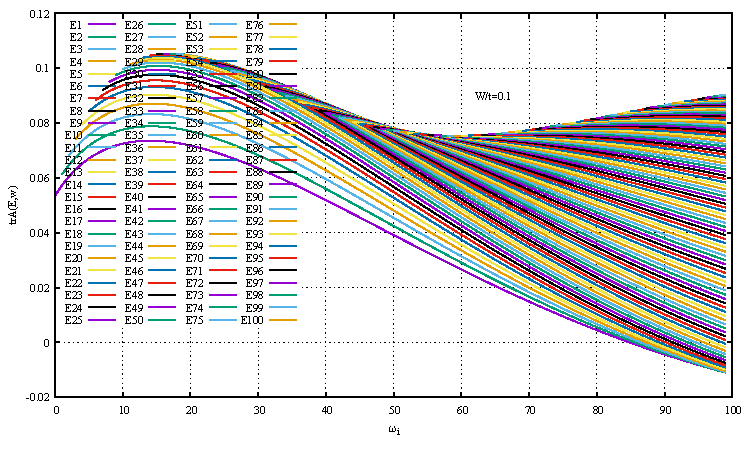
\includegraphics[width=8.5cm]{trA.pdf}
\caption{\label{fig:trA} $TrA$ for the clean NM-NM-FI system.}
\end{figure}

The interpolation to $trA$ reduces computation from 10000 points to 1000 points.








\begin{thebibliography}{10}
\bibitem{ref1}
Y, K, Kato. Observation of the Spin Hall Effect in Semiconductors[J]. Science, 2004.
\bibitem{CaoZhan}
Cao Zhan, Investigation on DC electronic transport in hybrid multiterminal quantum dot systems[D], 2017.
\end{thebibliography}

\end{document}
